\chapter{Řízení platformy}
\label{sec:PlatformControl}
\

Pro řízení platformy bylo použito 2 režimy řízení: automatický,
na základě algoritmu, a manuální, pomocí RC ovladače.
Přepínáni mezi režimy bylo implementováno
pomocí tlačítka na POLI-TFC.

\section{Dráha}
Testování řízení platformy bylo provedeno na draze ve tvaru osmičky.
Dráha je na obrázku \ref{fig:Road}

\begin{figure}[!htbp]
    \centering
    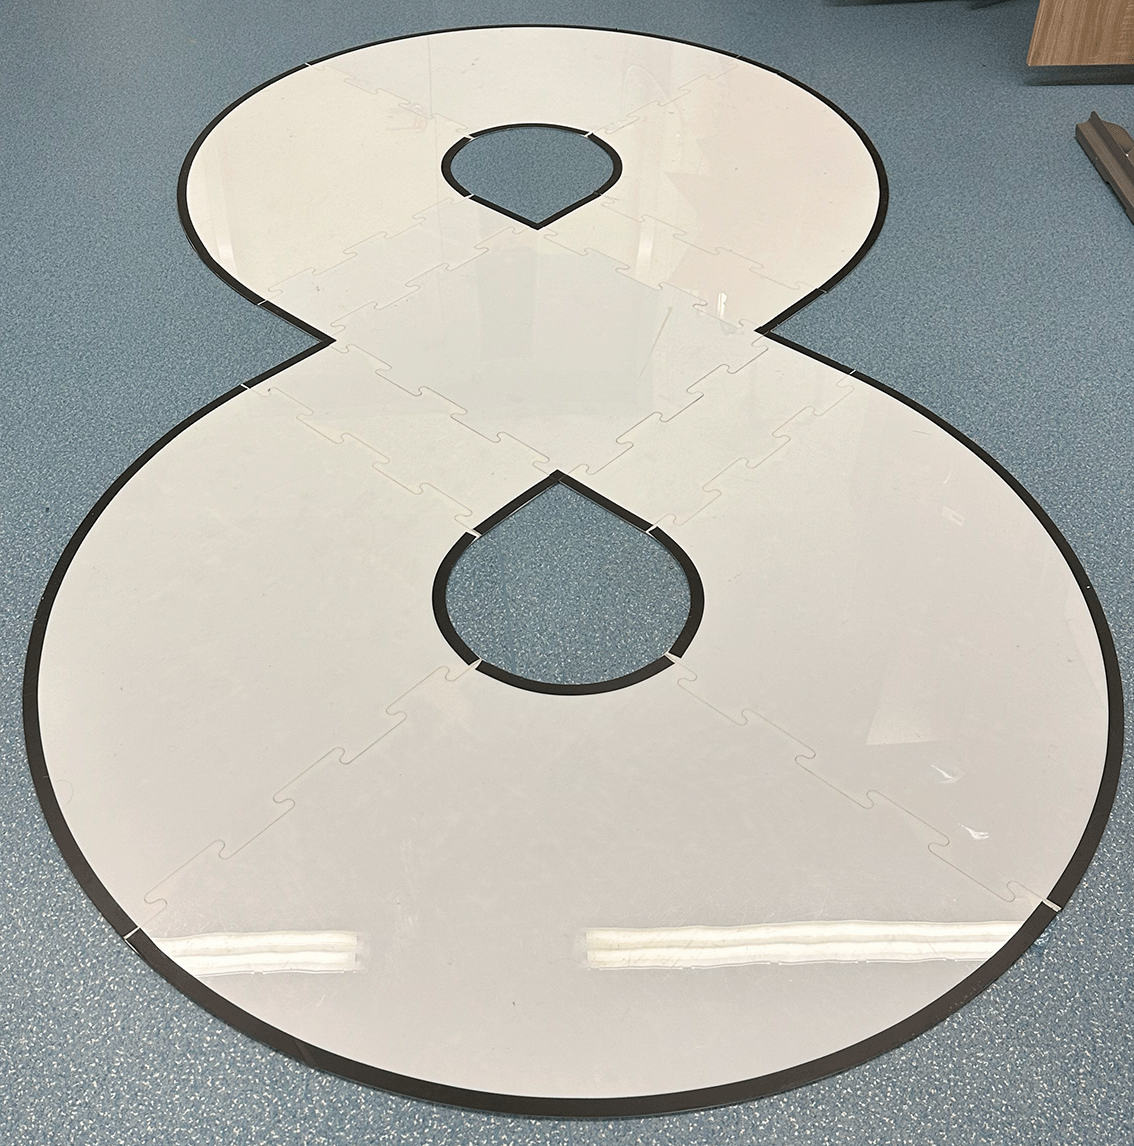
\includegraphics[width = 0.5\linewidth]{Figures/Road.png}
    \caption{Dráha.}
    \label{fig:Road}
\end{figure}

\section{Automatické řízení}\

Pro automatické řízení byly použity algoritmy rozpoznaní dráhy,
kontroly servomotoru a PWM~motorů.

\subsection{Rozpoznání dráhy}\

Pro získání obrazu dráhy se používá řádková kamera. Dále v programu
je použitá třída TFC\cite{draha}, která vrací data ve formátu 1D pole
typu uint16\_t (16 bitové celá čísla bez znaménka) v intervalu <0;4095>.

Obraz zpracovává v následujících krocích:
\begin{enumerate}
    \item Filtrování mediánem;
    \item Normalizace obrazu;
    \item Prahování průměrem.
\end{enumerate}

\subsubsection{Filtrování mediánem}\

Filtrování mediánem je užitečné pro odstranění malých artefaktu v obraze.
Filtr pracuje s pixelem a jeho okolím, proto potřebné uložit všichni okolní
pixely. Algoritmus je ve výpisu \ref{lst:slowMedianBlur}\cite{draha}\cite{robot}.

\begin{lstlisting}[caption=Filtrování mediánem, label=lst:slowMedianBlur]
// Image.cpp
void Image::slowMedianBlur(RefCImageLine srcImg, RefImageLine dstImg,
                           int pixels) {
    memcpy(dstImg, srcImg, LINE_LENGTH);
    std::vector<uint16_t> blurBuffer;

    for (int i = pixels; i < LINE_LENGTH - pixels; i++) {
        for (int j = -pixels; j <= pixels; j++) {
            blurBuffer.emplace_back(srcImg[i - j]);
        }
        std::sort(blurBuffer.begin(), blurBuffer.end());
        dstImg[i] = blurBuffer.at(pixels + 1);
        blurBuffer.clear();
    }
}
\end{lstlisting}


\subsubsection{Normalizace obrazu}\

Pro normalizace obrazu je potřebně najít hodnotu minimalního a maximalního bodu v
celém obraze. Normalizuje se každý bod z intervalu <min;max>
do intervalu <0;255>.

Díky normalizace obrazu auto je schopno přizpůsobit k různým světelným podmínkám.
Algoritmus normalizace je ve výpisu \ref{lst:normalize}\cite{robot}.
\begin{lstlisting}[caption=Normalizace obrazu, label=lst:normalize]
// Image.cpp
void Image::normalize(RefCImageLine srcImg, RefImageLine dstImg) const {
    for (int i = 0; i < LINE_LENGTH; i++) {
        auto pixel = static_cast<float>(srcImg[i]);
        pixel -= this->minValue;
        pixel *= COLOR_WHITE;
        pixel /= (this->maxValue - this->minValue);
        dstImg[i] = static_cast<uint16_t>(pixel);
    }
}
\end{lstlisting}

\subsubsection{Prahování průměrem}\

Pomocí prahování obraz se převadí do binárního, skládající z pouze dvou hodnot (0 a 1).
K tomu je nutno určit hodnotu prahu, se kterou se bude srovnávat každý pixel.
Pokud pixel je nižší než práh, je nastaven na 0, jinak nastaven na 1 nebo 255.
Algoritmus prahování průměrem je ve výpisu \ref{lst:threshold}\cite{robot}.
\begin{lstlisting}[caption=Prahování průměrem, label=lst:threshold]
// Image.cpp
void Image::threshold(RefCImageLine srcImg, RefImageLine dstImg) const {
    for (int i = 0; i < LINE_LENGTH; i++) {
        if (srcImg[i] < this->threshValue)
            dstImg[i] = COLOR_BLACK;
        else
            dstImg[i] = COLOR_WHITE;
    }
}
\end{lstlisting}

\subsection{Kontrola servomotoru}\

Pro kontrolu pozice servomotoru je použit PID regulátor. PID reguluje
zařízení tak, aby odchylka byla od nastavené hodnoty co nejmenší. Má 3 složky: proporcionální, integrační, derivativní\cite{PID}.

Pro proporcionální složku se používá rozdíl poměru vzdálenosti čar od okrajů obrazu.
\begin{lstlisting}[
	caption=Kalkulace poměru vzdálenosti čar,
	label=lst:calculateDistanceRatio
]
// Core.cpp
float Core::calculateDistanceRatio() {
    this->tracer.addImage(data.line);

    std::pair<uint8_t, uint8_t> distances = tracer.getDistancesPair();

    data.leftDistance = distances.first;
    data.rightDistance = Shared::Image::LINE_LENGTH - distances.second;

    const float leftRatio = static_cast<float>(data.leftDistance) /
                            static_cast<float>(data.rightDistance);
    const float rightRatio = static_cast<float>(data.rightDistance) /
                             static_cast<float>(data.leftDistance);

    data.regionsCount =
        tracer.getRegions(data.line, 0, TFC_CAMERA_LINE_LENGTH - 1, false).size();
    data.regionsListSize = tracer.listSize_;
    data.unchangedLeft = tracer.unchangedLeft_;
    data.unchangedRight = tracer.unchangedRight_;
    data.hasLeft = tracer.hasLeft_;
    data.hasRight = tracer.hasRight_;

    return rightRatio - leftRatio;
}
\end{lstlisting}

Hledaní těch čar implementováno pomocí algoritmu hledání tzv. Regionu.
Region je struktura, která uchovává indexy okrajů oblastí jedné barvy.
Algoritmus hledá regiony v smyčce, která si pamatuje barvu a porovná ji s barvou bodu.
Pokud barva se změnila, znamená to konec jednoho regionu a začátek nového.
Algoritmus je ve výpisu \ref{lst:getRegions}\cite{robot}.
\begin{lstlisting}[
	caption=Algoritmus hledání regionu,
	label=lst:getRegions
]
// LineTracer.cpp
std::vector<Shared::Region> LineTracer::getRegions(const Shared::Image &image, uint8_t searchLeftIdx, uint8_t searchRightIdx, bool saveToClass ) {
	std::vector<Shared::Region> foundRegions;

	uint8_t currentColor = static_cast<uint8_t>(image.atThresh(searchLeftIdx));
	foundRegions.emplace_back(Shared::Region({searchLeftIdx, searchLeftIdx, currentColor}));

	for (uint8_t i = searchLeftIdx; i <= searchRightIdx; i++) {
		if (currentColor != image.atThresh(i)) {
			if (foundRegions.size() > MAX_REGIONS_COUNT) {
				break;
			}
			foundRegions.at(foundRegions.size() - 1).right = i;
			foundRegions.emplace_back(Shared::Region({i, i, image.atThresh(i)}));
		}
		currentColor = static_cast<uint8_t>(image.atThresh(i));
	}

	if(saveToClass){
		currentRegions_ = foundRegions;
	}

	return foundRegions;
}
\end{lstlisting}

\subsection{Kontrola PWM motorů}\

Pro kontrolu motorů musíme rozlišovat dva režimy: zatáčení a jízda rovně.
Pro rozpoznaní zatáčení slouží algoritmus mediánu historie obrazu.
Aplikace si uchovává historii zpracovaných záznamů~(Regionů) a pro oba
okraje je vypočítán medián. Pokud se okraje aktuálního řídícího Regionu nachází
v blízkém okolí vypočteného mediánu, auto se pravděpodobně
nachází na rovině a oba motory se mohou otáčet na maximální nastavený výkon.
Pokud jinak, nachází se auto pravděpodobně v zatáčce a je tedy potřeba zpomalit
motor na straně, kde se nachází okraj.
Zpomalení implementováno na základě úhlu servomotoru.
Algoritmus je ve výpisu \ref{lst:getRegions}\cite{robot}.
\begin{lstlisting}[
	caption=Algoritmus kontroly PWM motorů\cite{robot},
	label=lst:controlPWM
]
// Core.cpp
float speed = SPEED;
data.angle = (data.servoPosition * 5.85f / 200) * PI /
	                 180.f; // Convert servo to angle

if (!(this->tracer.unchangedLeft_ && this->tracer.unchangedRight_)) {
    innerSpeed =
        speed * (1.f - DIFF_COEF * (1.50f * tanf(data.angle)) / 2.f * 1.85f);
    outerSpeed =
        speed * (1.f + DIFF_COEF * (1.50f * tanf(data.angle)) / 2.f * 1.85f);

    if (data.angle > 0.f) {
        data.rightSpeed = innerSpeed;
        data.leftSpeed = outerSpeed;
    } else {
        data.leftSpeed = innerSpeed;
        data.rightSpeed = outerSpeed;
    }

    data.servoPosition *= 1.5f;
    data.leftSpeed *= 0.75f;
    data.rightSpeed *= 0.75f;
} else {
    data.leftSpeed = speed;
    data.rightSpeed = speed;
}
\end{lstlisting}

\section{Manuální řízení}\

Pro manuální řízení byl použit ovladač OPTIC 6 SPORT (obrázek \ref{fig:Joystick}),
který posílá signál do přijímače Minima 6S.
Oba pracují na frekvence 2.4 GHz. Ovladač má
dvě páky. Jedna je použitá pro zvětšení a zmenšení plynu PWM motoru.
Druhá je použitá pro změnu pozice servomotoru\cite{RC}.

Oba signály jsou přijímány přes kanály CH1 a CH2\cite{RC}.
Tyto kanály jsou integrovány do modulu POLI-TFC shield,
kde jsou signály zpracovány programově prostřednictvím třídy TFC\cite{draha}.
Hodnoty signálů se nacházejí v rozsahu <1000;2000>, které jsou následně
transformovány do rozsahu <-1;1> pomocí níže uvedeného vzorce:

\begin{equation}
	\centering
	y = (x / 100 - 15) / 10,
\end{equation}

kde $y$ je normalizovaná hodnota a $x$ je hodnota z přijímače. Pak $y$ je násoben
na maximální hodnotu PWM motorů nebo servomotoru. Výsledek je použit pro
jejich nastaveni.

\begin{figure}[!h]
    \centering
    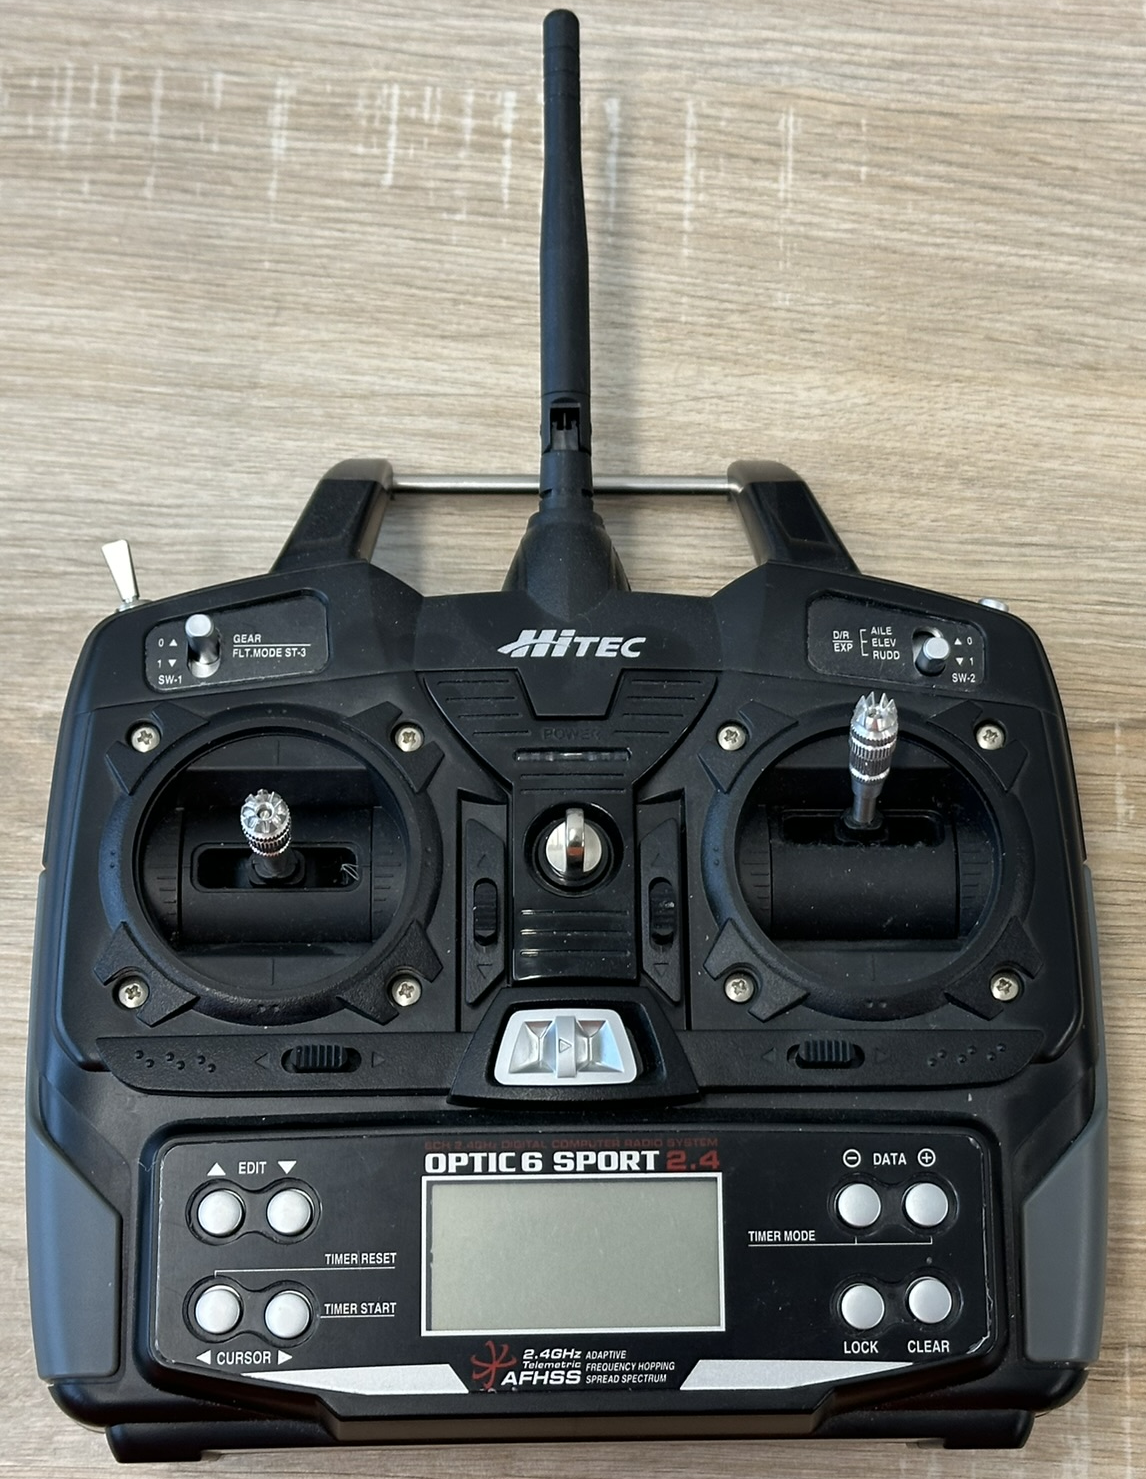
\includegraphics[width = 0.5\linewidth]{Figures/Joystick.png}
    \caption{Ovladač OPTIC 6 SPORT.}
    \label{fig:Joystick}
\end{figure}

\endinput
